%template1.tex
%The following LaTeX source file represents the simplest kind of slide presentation; no overlays, no included graphics. Substitute your favorite style for ``pascal''. To create the PDF file template1.pdf, (1) be sure to use the prosper class, then (2) execute the command latex template1.tex, and (3) the command dvipdf template1.dvi.

%%%%%%%%%%%%%%%%%%%%%%%%%%%%%%% template1.tex %%%%%%%%%%%%%%%%%%%%%%%%%%%%%%%%%%%
\documentclass[a4paper,blends,pdf,colorBG,slideColor]{prosper}
% definitions for slides for CSC544
% Lutz Hamel, (c) 2007

\hypersetup{pdfpagemode=FullScreen}

\usepackage{amssymb}
\usepackage{latexsym}
\usepackage{amsmath}
%\usepackage[usenames]{color}
\usepackage{xypic}


\newcommand{\term}[1]{\ensuremath{\mbox{\bf #1}}}
\newcommand{\nonterm}[1]{\ensuremath{\mbox{#1}}}
\newcommand{\ifstmt}[3]{\ensuremath{{\bf if}\; {#1}\;{\bf then}\;{#2}\;{\bf else}\;{#3}\;\term{end}}}
\newcommand{\whilestmt}[2]{\ensuremath{{\bf while}\; {#1}\;{\bf do}\;{#2}\; \term{end}}}
\newcommand{\funcstmt}[3]{\ensuremath{{\bf fun}\; {#1}\; {\bf is}\; {#2} \; {\bf return}\; {#3}}}
\newcommand{\syntaxset}[1]{\ensuremath{\mbox{\bf #1}}}
\newcommand{\orbar}{\;|\;}
\newcommand{\bs}[1]{\begin{slide}{#1}\ptsize{8}}
\newcommand{\es}{\end{slide}}
\newcommand{\co}{\,\colon\;}
\newcommand{\pair}[2]{\ensuremath{\langle {#1}, {#2} \rangle}}
\newcommand{\encode}[1]{\ensuremath{\langle {#1} \rangle}}
\newcommand{\mytab}{\makebox[.15in]{}}
%\newcommand{\abs}[1]{{\mid{#1}\mid}}
\newcommand{\abs}[1]{{|{#1}|}}
\newcommand{\ol}[1]{\overline{#1}}

\newcommand{\qaccept}{\ensuremath{q_{\mbox{\tiny accept}}}}
\newcommand{\qreject}{\ensuremath{q_{\mbox{\tiny reject}}}}
\newcommand{\accept}{{\em accept}}
\newcommand{\reject}{{\em reject}}

\newcommand{\machine}[1]{
	\begin{quote}
	{#1}
	\end{quote}
	}

\newcommand{\fdef}[1]{
	\begin{center}
	\fbox{
	\begin{minipage}{3.5in}
	{\bf Definition:}
	{#1}
	\end{minipage}
	}
	\end{center}
	}

\newcommand{\ftheorem}[1]{
	\begin{center}
	\fbox{
	\begin{minipage}{3.5in}
	{\bf Theorem:}
	{#1}
	\end{minipage}
	}
	\end{center}
	}

\newcommand{\flemma}[1]{
	\begin{center}
	\fbox{
	\begin{minipage}{3.5in}
	{\bf Lemma:}
	{#1}
	\end{minipage}
	}
	\end{center}
	}


\newcommand{\fframe}[1]{
	\begin{center}
	\fbox{
	\begin{minipage}{3.5in}
	{#1}
	\end{minipage}
	}
	\end{center}
	}

\newcommand{\nframe}[1]{
	\begin{center}
	\begin{minipage}{3.5in}
	{#1}
	\end{minipage}
	\end{center}
	}

\begin{document}

\bs{Approximations to $NP$ Solutions}
If we are faced with an $NP$ or $NP$-complete problem the best we can do on a
deterministic computer is a solution in exponential time.

Since exponential time solutions are impractical for obvious reasons we could consider approximations
to the actual solutions.

Here we look at approximation algorithms for the classic `Traveling Salesman Problem' ($TSP$).
\es

\bs{Traveling Salesman}
{\small
The idea is, given a set of cities (nodes) that are connected via roads (weighted edges), find the cheapest route through all the cities (find a Hamiltonian path that minimizes the sum of the weights
in the path).  Formally,

$TSP = \{ \encode{G,s,t,w} | G$ is directed weighted graph with a minimal Hamiltonian path of
weight $w$ from $s$ to $t \}.$
}
\es


\bs{Traveling Salesman}
{\small
\ftheorem{
\[
TSP \in \mbox{$NP$-hard}.
\]
}
{\bf Proof:}  Note, a problem is $NP$-hard if every $L \in NP$ can be reduced to it in polynomial time but the problem itself is not in $NP$.  No known $NP$ solution exists for $TSP$ ($NP$ problems have polynomial time verifiers; in $TSP$ it is not possible to verify a certificate in polynomial time).  It remains to show that all $L \in NP$ reduce to it in polynomial time.  We will show this by a polynomial time reduction  $f$ from $HAMPATH$  to $TSP$,
\[
\encode{G,s,t} \in HAMPATH \mbox{ iff } f(\encode{G,s,t}) \in TSP,
\]
where $f(\encode{G,s,t}) = \encode{G',s,t,m}$ with $G'$ the graph $G$ with a weight of $1$ on all of its edges
and $m$  the number of nodes in $G$.  Clearly, the reduction runs in polynomial time.  We verify the reduction condition by first observing that a Hamiltonian path gives rise to a minimal traveling salesman circuit by the virtue that all Hamiltonian paths in $G'$ have the same cost.  The converse also holds, if we have a traveling salesman circuit this implies that we have a Hamiltonian path. $\Box$
}
\es

\bs{Approximation Algorithms}
Approximation algorithms are an approach to attacking difficult optimization problems. Approximation algorithms are often associated with $NP$-hard problems. Since it is unlikely that there can ever be efficient (Polynomial Time) exact algorithms solving $NP$-complete/hard problems, one settles for non-optimal solutions, but requires them to be found in polynomial time. 

Unlike heuristics, which usually only find reasonably good solutions reasonably fast, one wants provable solution quality and provable run time bounds. Ideally, the approximation is optimal up to a small constant factor (say within 5\% of the optimal solution). It should be noted that approximation algorithms are increasingly being used for problems where polynomial algorithms are known but are too expensive due to the sizes of the data sets.
\es

\bs{A Heuristic}
A good heuristic is the {\bf\em nearest neighbor} algorithm.\footnote{{\tt http://en.wikipedia.org/wiki/Travelling\_salesman\_problem}}
\begin{quote}
$M$ = "On input $\encode{G}$, where $G$ is a directed weighted graph:
\begin{itemize}
\item[1.] Select node $s$ as the starting point.  Set $s$ as current node.
\item[2.] While there are unvisited nodes reachable from current node repeat:
\item[3.] \mytab Find out the lightest edge connecting current node and a unvisited node $v$.
\item[4.] \mytab Set current node to be $v$.
\item[5.] \mytab Mark $v$ as visited.
\item[6.] If all nodes have been visited, \accept; otherwise, \reject."
\end{itemize}
\end{quote}
In general, this heuristic provides a circuit with length $log(m)*t$, where $m$ is the number of nodes in the graph and $t$ the optimal circuit.  But this bound is not guaranteed.
\es

\bs{An Approximation Algorithm}
\vspace{.2in}
\fdef{(Triangle Inequality)
The property that a complete weighted graph satisfies $weight(u,v) \le weight(u,w) + weight(w,v)$ for all vertices $u, v, w$. (Informally, the graph has no short cuts. )
}
\vspace{.5in}
(source: www.itl.nist.gov)
\es

\bs{An Approximation Algorithm}

Minimum Spanning Tree: The algorithm continuously increases the size of a tree starting with a single vertex until it spans all the vertices.

\begin{itemize}
\item Input: A connected weighted graph with vertices $V$ and edges $E$.
\item Initialize: $V_{\text{new}} = \{s\}$, where $s$ is an arbitrary node (starting point) from $V$; $E_{\text{new}} = \{ \}$.
\item Repeat until $V_{\text{new}} = V$:
	\begin{itemize}
          \item Choose edge $(u,v)$ from $E$ with minimal weight such that $u$ is in $V_{\text{new}}$ and $v$ is not (if there are multiple edges with the same weight, choose arbitrarily)
          \item Add $v$ to $V_{\text{new}}$, add $(u, v)$ to $E_{\text{new}}$
	\end{itemize}
\item Output: $V_{\text{new}}$ and $E_{\text{new}}$ describe a minimal spanning tree.
\end{itemize}

Runs in $O(V^2)$ time.
\es



\bs{An Approximation Algorithm}
Assume that the directed graph $G$ is fully connected and the triangle inequality is satisfied.  Then we can use the following algorithm to
compute an approximate solution to the $TSP$ problem.

\begin{quote}
$M$ = "On input $\encode{G}$, where $G$ is a directed fully connected weighted graph:
\begin{itemize}
\item[1.] Select node $s$ as the start node for the circuit.
\item[2.] Construct a minimum-cost spanning tree rooted in $s$.
\item[3.] Construct a sequence of nodes visited by a preorder traversal of the spanning tree.
\item[4.] Delete nodes that occur more than once in the sequence.
\item[5.] \accept."
\end{itemize}
\end{quote}

The triangle equality and the fully-connectedness assures that we can build the circuit.  It can be shown that the cost of the computed circuit is bounded by twice the cost of the minimal spanning tree.

\es


\bs{An Approximation Algorithm}
\begin{center}
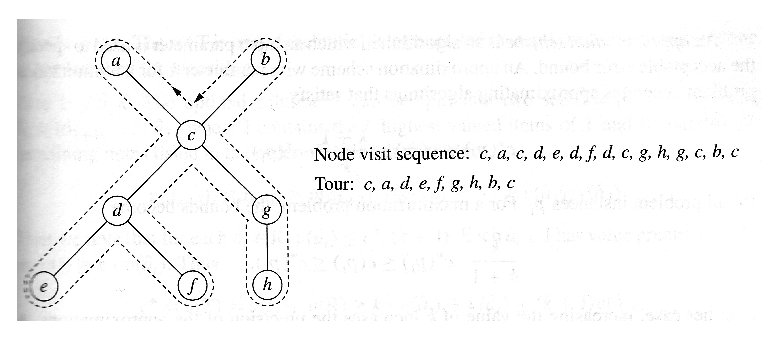
\includegraphics[height=50mm]{images/tsp.eps}
\end{center}
\es

\bs{\large Approximations to $P$ Solutions: Probabilistic Machines}
Here is our first extension to traditional TM's

\fdef{ A {\em\bf probabilistic Turing machine} $M$ is a type of nondeterministic Turing machine
in which each nondeterministic step is called a {\em\bf coin-flip step} and has two legal next moves.
We assign a probability to each branch $b$ of $M$'s computation on input $w$ as follows.
Define the probability of branch $b$ to be
\[
Pr[b] = 2^{-i},
\]
where $i$ is the number of coin-flip steps that occur in branch $b$.
Define the probability that $M$ accepts $w$ to be 
\[
Pr[\text{$M$ accepts $w$}] = \sum_{\text{$b$ is an accepting branch}} Pr[b].
\]
Furthermore,
\[
Pr[\text{$M$ rejects $w$}]  = 1 - Pr[\text{$M$ accepts $w$}].
\]
}
\es

\bs{Probabilistic Machines}
Our definition implies the following: When a probabilistic TM recognizes a language then it must
accept all strings in the language and reject all strings not in the language with the exception that
now we allow the machine to make errors with some small probability.

For $0 \le \epsilon < 1/2$ we say that {\em\bf $M$ recognizes language $A$ with error probability $\epsilon$} if
\begin{enumerate}
\item $w \in A$ implies $Pr[\text{$M$ accepts $w$}] \ge 1 - \epsilon$, and
\item $w \not\in A$ implies $Pr[\text{$M$ rejects $w$}] \ge 1 - \epsilon$.
\end{enumerate}
That is, the probability that we obtain a wrong answer is at most $\epsilon$.
\es

\bs{Amplification Lemma}
\small
The following lemma allows us to make the error on a probabilistic machine as small as desired.

\flemma{(Amplification Lemma) Let $\epsilon$ be a fixed constant strictly between 0 and $1/2$, then
for any polynomial $f(n)$ a probabilistic polynomial time TM $M_1$ that operates with error 
probability $\epsilon$ has an equivalent probabilistic polynomial time TM $M_2$ that operates with
an error probability of $2^{-f(n)}$.
}


{\bf Proof Sketch:} The machine $M_2$ runs the machine $M_1$ $k$ number of times where $k$ is
picked such that the error probability $2^{-f(n)}$ holds.  The outcome of the machine is determined by
majority vote.
\begin{quote}
$M_2$ = "On input $w$:
\begin{itemize}
\item[1.] Calculate $k$ (see below).
\item[2.] Run $2k$ independent simulations of $M_1$ on $w$.
\item[3.] If most runs accept, the \accept; otherwise \reject.
\end{itemize}
\end{quote}
We can compute $k$ as
\[
k \ge \frac{f(n)}{\log_2(4\epsilon(1-\epsilon))},
\]
where $f(n) \ge 1$.
\es

\bs{Monte-Carlo Algorithms}

\vspace{.2in}
Given a language $A$ recognized by  a probabilistic TM $M$, we say that $M$ is a Monte-Carlo algorithm, if
\begin{enumerate}
\item $w \in A$ implies $Pr[\text{$M$ accepts $w$}] \ge 1/2$, and
\item $w \not\in A$ implies $Pr[\text{$M$ rejects $w$}] = 1$.
\end{enumerate}

This gives rise to a new complexity class called {\em\bf Randomized Polynomial} time algorithms, $RP$.

\fdef{$RP$ is the class of languages that are recognized by probabilistic polynomial time TMs where
the inputs in the language are accepted with a probability of at least $1/2$ and input not in the language are 
rejected with probability of 1.}

From a theoretical point of view these algorithms are barely distinguishable from $P$.  However, from a
practical point of view Monte-Carlo algorithms allow us to compute solutions in $P$ that are otherwise too complex.
\es

\bs{Monte-Carlo Algorithms}
\small
{\bf Example:}The Triangle decision problem.  A graph is in Triangle if it contains a 3-clique.
This problem is in $P$ with $O(n^3)$.  We can construct a Monte-Carlo algorithm $M$ for this problem: (a) pick an edge $(v,u) \in E$ with $v,u\in V$ and a vertex $p\in V$
such that $p \ne v$ and $p \ne u$.  If $(u,v,p)$ form a triangle accept otherwise reject.  (b) perform step (a) $k$ times and accept if at least one of the iterations accepts.

In order to verify that this algorithm is Monte-Carlo we have to verify the conditions
\begin{enumerate}
\item $\langle G \rangle \in \text{Triangle}$ implies $Pr[\text{$M$ accepts $\langle G \rangle$}] \ge 1/2$, and
\item $\langle G \rangle \not\in \text{Triangle}$ implies $Pr[\text{$M$ rejects $\langle G \rangle$}] = 1$.
\end{enumerate}

Condition 1 can be shown to be fulfilled by the algorithm if we pick $k = \abs{E}(\abs{V} - 2)/3$.

Condition 2 is easily verified; the algorithm cannot accept a graph with no triangle, all experiments fail.

\es
\end{document}
%%%%%%%%%%%%%%%%%%%%%%%%%%% end of template1.tex %%%%%%%%%%%%%%%%%%%%%%%%%%%%%%%%

